\begin{enumerate}
	\item Exercício retirado da página 1023 de \cite{James_Stewart_calculo_v2}
	
	Determine o volume da região $E$ limitada pelos paraboloides $z = x^2 + y^2$ e $z = 36-3x^2-3y^2$.
	
	\begin{figure}[htb]
		\caption{Coordenadas cilíndricas - Aula 07 - Exercício I}
		\label{v31_a07_e01}
		\centering
		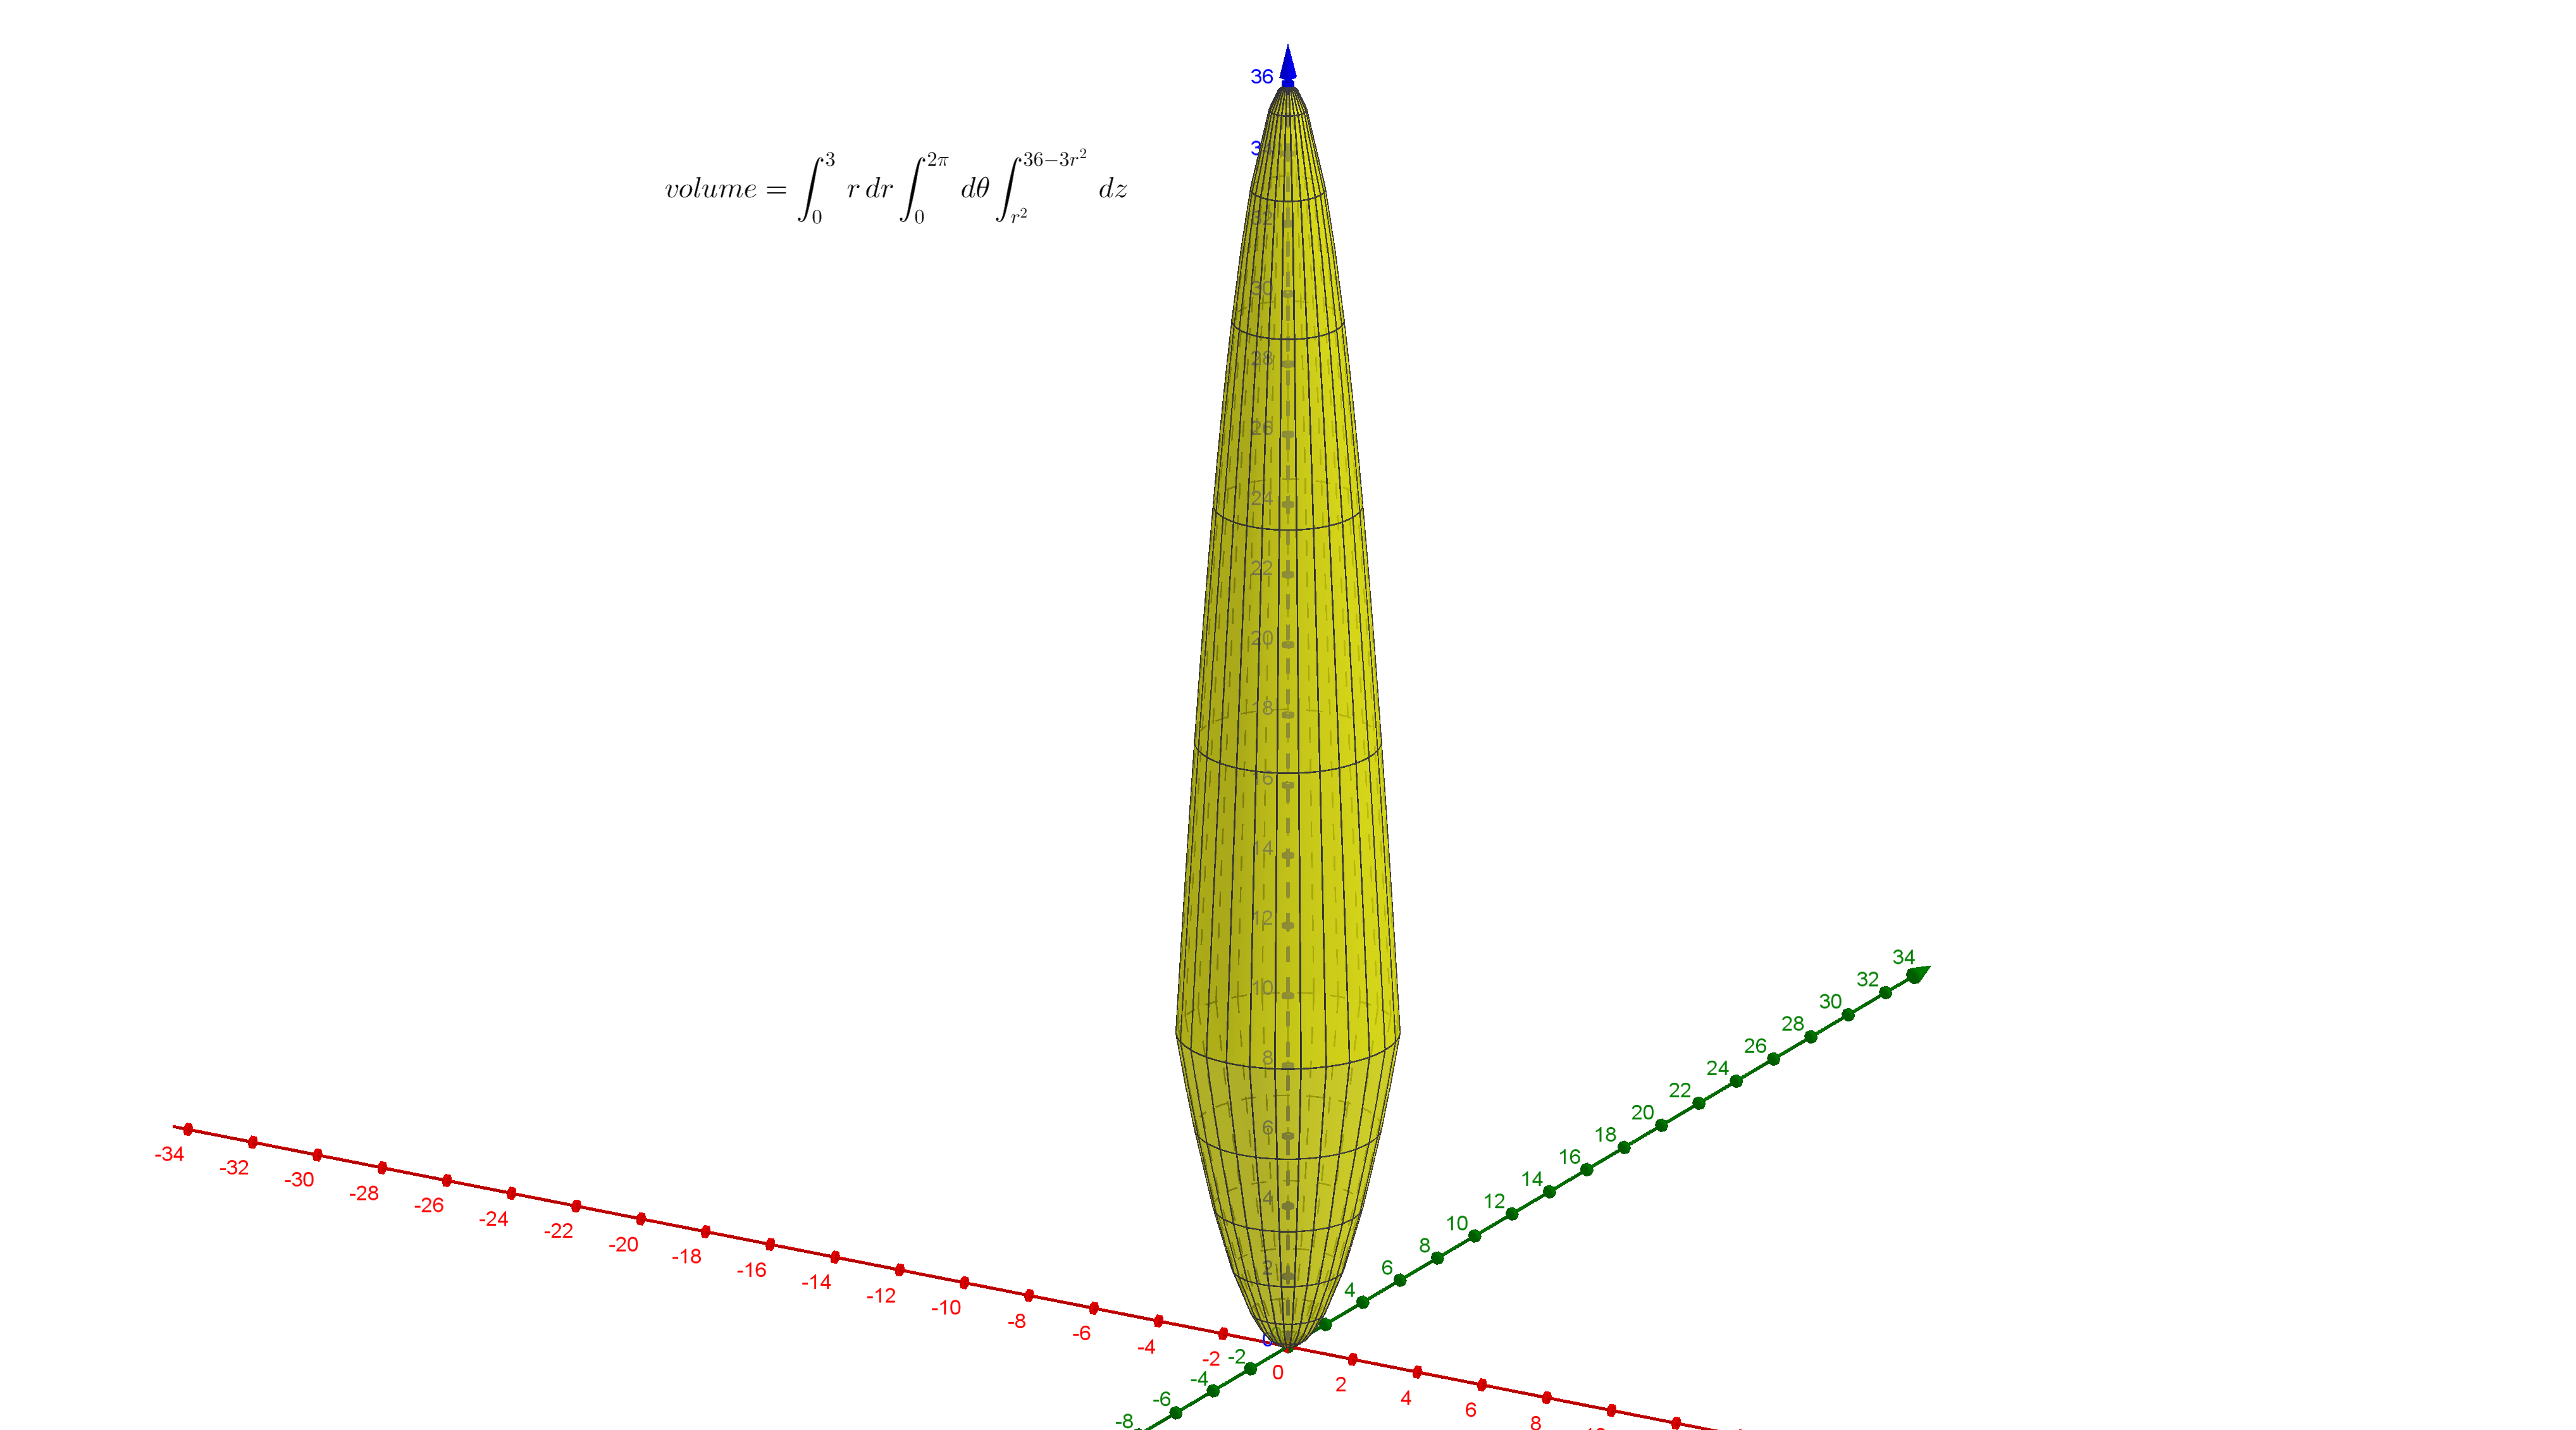
\includegraphics[width=0.5\textwidth]{v31_a07_e01.png}		
	\end{figure}
	
	\begin{equation*}
		z = x^2 + y^2 = r^2
	\end{equation*}
	\begin{equation*}
		z = 36-3x^2-3y^2 = 36-3\left(x^2 + y^2\right) = 36-3r^2
	\end{equation*}
	\begin{equation*}
		r^2 = 36-3r^2 \Rightarrow r^2 + 3r^2 = 36 \Rightarrow 4r^2 = 36 \Rightarrow r^2 = \dfrac{36}{4} = 9 \Rightarrow r = \sqrt{9} = 3
	\end{equation*}
	\begin{equation*}
		0 \leq r \leq 3,\, 0 \leq \theta \leq 2\pi,\, r^2 \leq z \leq 36-3r^2
	\end{equation*}
	\begin{gather*}
		\int_0^3 \int_0^{2\pi} \int_{r^2}^{36-3r^2} r\, dz d\theta dr = \int_0^3 r\, dr \int_0^{2\pi} d\theta \int_{r^2}^{36-3r^2} dz = \int_0^3 r\, dr \int_0^{2\pi} d\theta \left[z\right]_{r^2}^{36-3r^2} =\\ \int_0^3 r\, dr \int_0^{2\pi} d\theta \left[36-3r^2-r^2\right] = \int_0^3 r\, dr = \int_0^3 r\left(36-4r^2\right)\, dr \int_0^{2\pi} d\theta  = \int_0^3 r\, dr =\\ \int_0^3 \left(36r-4r^3\right)\, dr \int_0^{2\pi} d\theta = \left[\dfrac{36r^2}{2} - \dfrac{4r^4}{4}\right]_0^3 \left[\theta\right]_0^{2\pi} = 2\pi \left[18r^2 - r^4\right]_0^3 =\\ 2\pi \left(18\cdot 3^2 - 3^4\right) = 2\pi\left(162 - 81\right) = 162\pi
	\end{gather*}
\end{enumerate}